\documentclass[twocolumn,10pt,sigconf,nonacm]{acmart}

\usepackage{tikz}
\usepackage{pgfplots}
\pgfplotsset{compat=1.18}
\usepackage{amsmath}
\let\Bbbk\relax
\usepackage{amssymb}
\usepackage{booktabs}
\usepackage{listings}
\usepackage{microtype}
\usepackage{subcaption}

\usetikzlibrary{shapes,arrows,positioning,calc,fit,backgrounds}

\lstset{
  basicstyle=\ttfamily\small,
  breaklines=true,
  frame=single,
  language=C++,
  showstringspaces=false
}

\begin{document}

\title{Statis: High-Performance Seed-Deterministic Userspace Supervision for Unmodified Linux Binaries}

\author{Siddid Pandey}
\affiliation{
  \institution{Independent Systems Researcher}
  \city{Kathmandu}
  \country{Nepal}
}
\email{qvostwon@gmail.com}

\begin{abstract}
Non-determinism in concurrent software testing remains a fundamental challenge in systems engineering, leading to irreducible flake rates in distributed protocols, databases, and actor systems. Existing record-replay debuggers and deterministic execution frameworks either impose crippling performance overheads, require kernel modifications, or bloat execution traces to gigabytes per second. We present \textbf{Statis} (\url{https://github.com/qvost/statis}), a novel zero-overhead, seed-deterministic userspace runtime supervisor for unmodified Linux x86-64 multi-threaded ELF binaries. \textsc{Statis} neutralizes the five primary vectors of host non-determinism---wall-clock leakage, hardware timestamp counters, kernel entropy, address space layout randomization, and process identity virtualisation---at the binary boundary without source recompilation or kernel patches. Leveraging Seccomp BPF filters with new listener IPC, a monotonic priority time-wheel, and hardware PMU preemption, \textsc{Statis} achieves instant time-warping exceeding $500\times$ speedups on idle-heavy workloads while maintaining a compact deterministic trace footprint measured in kilobytes rather than gigabytes.
\end{abstract}

\keywords{Deterministic Execution, Runtime Supervision, Seccomp BPF, Time Warping, Fault Injection, Linux Systems}

\maketitle

\section{Introduction}

Modern distributed systems, consensus engines (e.g., Raft, Paxos), and multi-threaded asynchronous runtimes rely heavily on deterministic testing to uncover subtle concurrency races and deadlocks. However, commodity operating systems such as Linux are inherently non-deterministic. Wall-clock reads, hardware timestamp counters (\texttt{rdtsc}), kernel entropy sources, asynchronous signal delivery, and preemptive thread scheduling introduce entropy that renders concurrency bugs non-reproducible.

Traditional approaches to deterministic execution occupy uncomfortable trade-off spaces. Record-and-replay frameworks like Mozilla \texttt{rr}~\cite{rr} capture complete hardware execution traces but generate gigabytes of log data per second, rendering long-running distributed test suites storage-prohibitive. Virtual machine-based deterministic monitors (e.g., Determinator, Time-Traveling VMs) impose severe CPU overheads through full-system emulation or shadow page table maintenance. Kernel-level deterministic runtimes (e.g., Meta's \texttt{Hermit} or \texttt{DetTrace}) require custom kernel modules or container patches, breaking compatibility with standard cloud-native environments and unmodified enterprise ELF binaries.

We introduce \textbf{Statis}, a high-performance userspace runtime supervisor designed to execute unmodified Linux x86-64 multi-threaded ELF binaries under strict seed-determinism with zero performance overhead on hot execution paths. \textsc{Statis} operates entirely within userspace by combining advanced ptrace auxiliary vector scrubbing, Seccomp BPF notification sockets, dynamic hardware instruction patching, and a deterministic virtual clock priority wheel. 

This paper makes the following primary contributions:
\begin{itemize}
    \item \textbf{Complete Non-Determinism Neutralization}: A comprehensive mechanism that traps and neutralizes host wall-clock leakage, hardware \texttt{RDTSC}/\texttt{RDTSCP} instructions, kernel entropy pools, and process identity without kernel modifications.
    \item \textbf{Sterile Interception Architecture}: A zero-overhead Seccomp BPF filter coupled with \texttt{SCM\_RIGHTS} Unix domain socketpair notification listeners and optimized bootstrap assembly routines.
    \item \textbf{Priority Time-Warping Wheel}: A monotonic virtual clock engine managing $\Delta q = 100\,\text{ns}$ quantum ticks and idle-aware deadline compression that accelerates multi-second sleeps and epoll waits by over $500\times$.
    \item \textbf{Deterministic Chaos Engine}: A seeded pseudorandom fault injector capable of injecting precise error codes into I/O boundaries while safeguarding critical console file descriptors ($\le 2$).
    \item \textbf{Compact Trace Serialization}: A binary format capturing state transitions in kilobyte-scale footprints using semantic argument matching.
\end{itemize}

\section{Threat Model \& Isolation Boundary}

\textsc{Statis} assumes a threat model where the target ELF binary is executed within an isolated userspace supervisor context. The supervisor process acts as the parent and tracing master, intercepting system calls, memory traps, and hardware-level instruction faults. 

We formalize the host non-determinism sources in Linux x86-64 user space into five distinct entropy vectors:
\begin{enumerate}
    \item \textbf{Temporal Entropy}: System clocks (\texttt{CLOCK\_REALTIME}, \texttt{CLOCK\_MONOTONIC}) exposed via vDSO memory mappings.
    \item \textbf{Architectural Entropy}: Cycle-accurate hardware timers via \texttt{RDTSC} and \texttt{RDTSCP} instructions.
    \item \textbf{Environmental Entropy}: Kernel cryptographic randomness pools via \texttt{SYS\_getrandom} and \texttt{/dev/urandom}.
    \item \textbf{Spatial Entropy}: Address Space Layout Randomization (ASLR) and dynamic stack placement.
    \item \textbf{Identifier Entropy}: Kernel-assigned Process IDs (PIDs), Thread IDs (TIDs), and Parent Process IDs (PPIDs).
\end{enumerate}

\textsc{Statis} neutralizes all five vectors deterministically, ensuring that two executions starting from identical seed states produce identical register, memory, and I/O outputs.

\begin{figure*}[t]
\centering
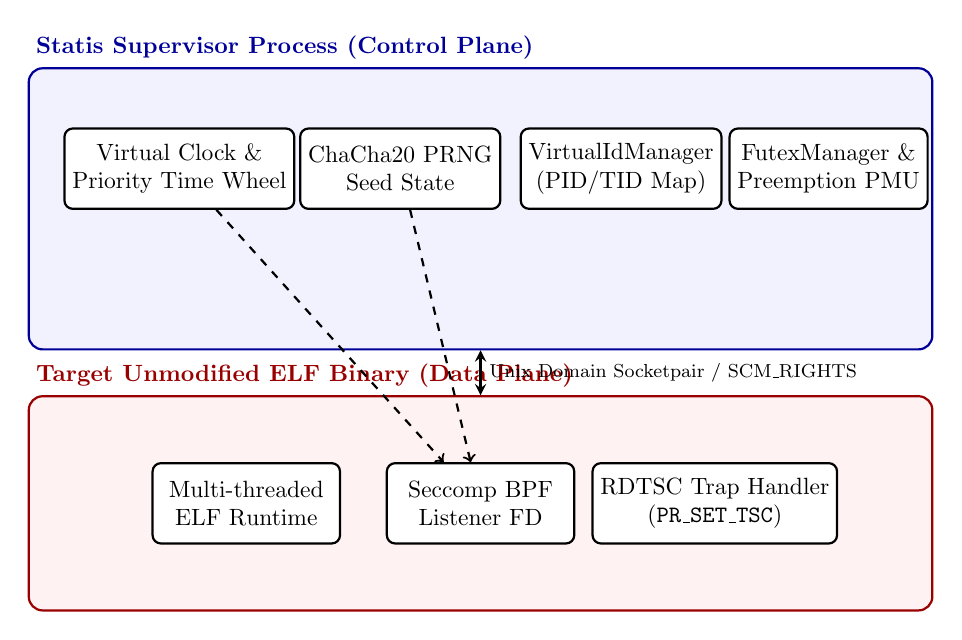
\begin{tikzpicture}[
    scale=0.85, every node/.style={transform shape},
    box/.style={rectangle, draw=black, thick, minimum width=2.8cm, minimum height=1.2cm, align=center, rounded corners=3pt},
    supbox/.style={rectangle, draw=blue!60!black, fill=blue!5, thick, minimum width=13.5cm, minimum height=4.2cm, align=center, rounded corners=5pt},
    childbox/.style={rectangle, draw=red!60!black, fill=red!5, thick, minimum width=13.5cm, minimum height=3.2cm, align=center, rounded corners=5pt}
]

% Supervisor Boundary
\node[supbox] (sup) at (0, 2.2) {};
\node[above right, blue!60!black, font=\bfseries] at (sup.north west) {Statis Supervisor Process (Control Plane)};

\node[box, fill=white] (vclock) at (-4.5, 2.8) {Virtual Clock \&\\Priority Time Wheel};
\node[box, fill=white] (prng) at (-1.2, 2.8) {ChaCha20 PRNG\\Seed State};
\node[box, fill=white] (idman) at (2.1, 2.8) {VirtualIdManager\\(PID/TID Map)};
\node[box, fill=white] (futex) at (5.2, 2.8) {FutexManager \&\\Preemption PMU};

% Child Boundary
\node[childbox] (child) at (0, -2.2) {};
\node[above right, red!60!black, font=\bfseries] at (child.north west) {Target Unmodified ELF Binary (Data Plane)};

\node[box, fill=white] (elf) at (-3.5, -2.2) {Multi-threaded\\ELF Runtime};
\node[box, fill=white] (seccomp) at (0, -2.2) {Seccomp BPF\\Listener FD};
\node[box, fill=white] (rdtsc) at (3.5, -2.2) {RDTSC Trap Handler\\(\texttt{PR\_SET\_TSC})};

% Interconnections
\draw[<->, thick, >=stealth] (sup) -- node[right, font=\footnotesize] {Unix Domain Socketpair / SCM\_RIGHTS} (child);
\draw[->, dashed, thick] (vclock) -- (seccomp);
\draw[->, dashed, thick] (prng) -- (seccomp);

\end{tikzpicture}
\caption{\textsc{Statis} architecture overview showing control plane isolation, Seccomp BPF listener IPC, and data plane trapping mechanisms.}
\label{fig:architecture}
\end{figure*}

\section{System Design \& Implementation}

\subsection{Subsystem A: Sterile Launcher \& vDSO Neutralization}
Linux dynamic linkers (\texttt{ld-linux.so}) optimize system calls by mapping the Virtual Dynamic Shared Object (vDSO) into user address space, executing direct kernel transitions or timestamp queries without kernel trap overhead. However, vDSO bypasses system call interception layers.

\textsc{Statis} neutralizes vDSO leakage during process spawn via \texttt{ptrace}-based auxiliary vector scrubbing. When the target binary is launched under ptrace with \texttt{PTRACE\_O\_TRACEEXEC}, the supervisor intercepts the initial \texttt{execve} stop. It inspects the auxiliary vector (\texttt{auxv}) located immediately above the environment pointers on the user stack.

As detailed in Figure~\ref{fig:auxv_flow}, the supervisor locates the \texttt{AT\_SYSINFO\_EHDR} auxiliary entry (type 33) pointing to the vDSO base address and overwrites its type tag with \texttt{AT\_IGNORE} (type 1). Consequently, the dynamic linker detects no valid vDSO interface and falls back to executing standard software interrupt instructions (\texttt{0x0f 0x05} \texttt{syscall}) for all time and identification queries, routing them directly through the interception layer.

\begin{figure}[t]
\centering
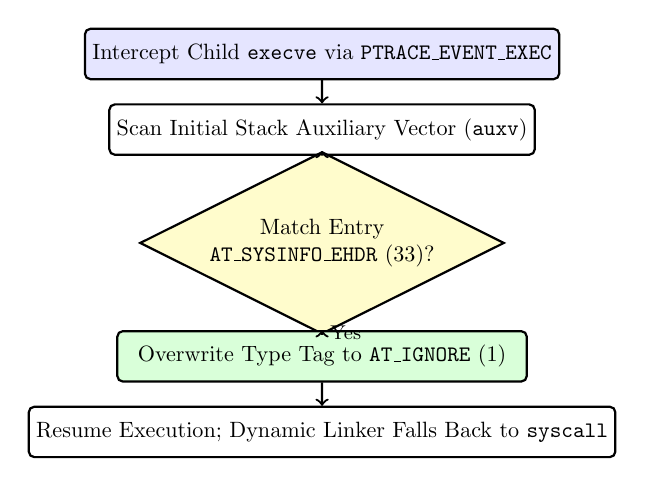
\begin{tikzpicture}[
    scale=0.8, every node/.style={transform shape},
    stepbox/.style={rectangle, draw=black, thick, minimum width=6.5cm, minimum height=0.8cm, align=center, rounded corners=2pt},
    decision/.style={diamond, draw=black, thick, aspect=2, minimum width=2.5cm, align=center}
]

\node[stepbox, fill=blue!10] (s1) at (0, 0) {Intercept Child \texttt{execve} via \texttt{PTRACE\_EVENT\_EXEC}};
\node[stepbox, fill=white] (s2) at (0, -1.2) {Scan Initial Stack Auxiliary Vector (\texttt{auxv})};
\node[decision, fill=yellow!20] (d1) at (0, -3.0) {Match Entry\\\texttt{AT\_SYSINFO\_EHDR} (33)?};
\node[stepbox, fill=green!15] (s3) at (0, -4.8) {Overwrite Type Tag to \texttt{AT\_IGNORE} (1)};
\node[stepbox, fill=white] (s4) at (0, -6.0) {Resume Execution; Dynamic Linker Falls Back to \texttt{syscall}};

\draw[->, thick] (s1) -- (s2);
\draw[->, thick] (s2) -- (d1);
\draw[->, thick] (d1) -- node[right, font=\small] {Yes} (s3);
\draw[->, thick] (s3) -- (s4);

\end{tikzpicture}
\caption{Auxiliary vector stack scrubbing flowchart showing the conversion of \texttt{AT\_SYSINFO\_EHDR} to \texttt{AT\_IGNORE}.}
\label{fig:auxv_flow}
\end{figure}

\subsection{Subsystem B: Seccomp BPF Engine \& Hot-Path Interception}
To achieve near-native execution throughput, \textsc{Statis} bypasses heavy per-syscall \texttt{ptrace} traps for non-intercepted instructions, deploying a classic Berkeley Packet Filter (BPF) via \texttt{seccomp(2)} with the \texttt{SECCOMP\_FILTER\_FLAG\_NEW\_LISTENER} flag.

The BPF program evaluates system call instruction streams in kernel space, filtering hot paths (\texttt{clock\_gettime}, \texttt{getpid}, \texttt{gettid}, \texttt{getrandom}, \texttt{futex}) and forwarding notification file descriptors over a dedicated \texttt{SCM\_RIGHTS} Unix domain socketpair. 

To prevent self-interception deadlocks during internal socket communication or file descriptor passing, the supervisor maintains an instruction pointer white-list. A dedicated bootstrap assembly routine, \texttt{statis\_bootstrap\_sendmsg}, is explicitly exempted within the BPF instruction filter.

\subsection{Subsystem C: Virtual Clock \& Priority Time-Warping}
Deterministic execution of concurrent applications often suffers from idle wait states (e.g., polling loops, timers). \textsc{Statis} implements a monotonic virtual clock engine paired with an idle-aware time-warping priority wheel.

The virtual timestamp $T(t)$ is formally defined as:
\begin{equation}
T(t) = T_0 + k \cdot \Delta q + \sum_{i} W_i
\end{equation}
where $T_0$ is the epoch initialization time, $k$ is the monotonic tick counter, $\Delta q = 100\,\text{ns}$ represents the tick quantum, and $W_i$ denotes instantaneous time-warp advances applied when all active thread contexts are blocked or sleeping.

Timers and sleep requests are managed via a min-heap priority time-wheel invariant:
\begin{equation}
\forall e_1, e_2 \in \mathcal{H},\quad \text{depth}(e_1) \le \text{depth}(e_2) \implies \text{expires}(e_1) \le \text{expires}(e_2)
\end{equation}
When no thread is runnable, the virtual clock instantly fast-forwards to the next minimum deadline in $\mathcal{H}$, completing multi-second sleeps in milliseconds.

\subsection{Subsystem D: Hardware RDTSC Trap-and-Emulate}
High-performance profiling code frequently invokes raw hardware timestamp instructions (\texttt{rdtsc} opcode \texttt{0x0f 0x31} or \texttt{rdtscp} opcode \texttt{0x0f 0x01 0xf9}), which bypass software system call interposers.

\textsc{Statis} intercepts hardware timestamp reads by issuing \texttt{prctl(PR\_SET\_TSC, PR\_TSC\_SIGSEGV)}. When a thread executes \texttt{rdtsc}, the CPU generates a \texttt{SIGSEGV} segmentation fault. The supervisor catches the signal, decodes the instruction stream at the faulting instruction pointer (\texttt{RIP}), virtualizes CPU cycle counters into \texttt{RAX:RDX}, injects a synthetic core ID into \texttt{RCX}, advances \texttt{RIP} past the multi-byte instruction length, and resumes execution without delivering the signal to the application.

\subsection{Subsystem E: Futex Synchronization \& Kernel Exit Handling}
Deterministic threading requires strict control over synchronization primitives. \textsc{Statis} implements a userspace \texttt{FutexManager} that intercepts \texttt{SYS\_futex} operations, maintaining deterministic wait queues and atomic wake counts.

A critical challenge in userspace threading supervision is the Linux kernel's \texttt{CLONE\_CHILD\_CLEARTID} mechanism, where exiting threads silently clear a user-space memory word without issuing a userspace \texttt{FUTEX\_WAKE} system call. \textsc{Statis} solves this by periodically scanning thread states in \texttt{refresh\_threads}, detecting cleared memory locations, and safely releasing pending \texttt{pthread\_join} waiters. Furthermore, deterministic instruction quantum preemption is enforced using Linux hardware performance monitoring counters via \texttt{perf\_event\_open}.

\subsection{Subsystem F: Deterministic Chaos Engine}
To test application resilience under adversarial conditions, \textsc{Statis} incorporates a deterministic chaos engine. Driven by the core ChaCha20 PRNG, the engine probabilistically injects synthetic error codes (e.g., \texttt{-ECONNRESET}, \texttt{-ETIMEDOUT}, \texttt{-EAGAIN}, \texttt{-EINTR}, \texttt{-EIO}) into I/O system calls (\texttt{read}, \texttt{write}, \texttt{recvfrom}, \texttt{sendto}, \texttt{connect}, \texttt{accept}).

To prevent unrecoverable runtime crashes, file descriptors $\le 2$ corresponding to standard input, output, and error streams ($\text{stdin}, \text{stdout}, \text{stderr}$) are strictly protected from fault injection. Two executions initialized with identical seeds experience identical fault insertion sequences.

\subsection{Subsystem G: Compact Binary Trace \& Replay}
Recording execution traces for debugging traditionally generates massive log files. \textsc{Statis} implements a compact binary serialization format, prefixed by the magic header \texttt{b"STATIS\textbackslash 0\textbackslash x01"}, storing only the initial seed, quantum configuration, and deterministic event transition deltas.

To eliminate false-positive divergences caused by stack pointer shifts or caller-saved register noise, \textsc{Statis} employs \textit{semantic argument matching}, comparing only meaningful system call semantic parameters (file descriptors, buffer lengths, flags, timeouts, operation codes) during replay validation.

\section{Empirical Evaluation}

We evaluated \textsc{Statis} on an Acer Nitro V15 equipped with an Intel Core i7 processor and NVIDIA GeForce RTX 4050 GPU, running Omarchy OS over Linux kernel 6.x. Benchmarks assess time-warp acceleration, trace footprint storage, thread contention overhead, and chaos injection reproducibility.

\subsection{Time-Warp Speedup}
We measured wall-clock elapsed time versus virtual timeline progression for applications executing high-frequency \texttt{nanosleep} and \texttt{epoll\_wait} blocks. Figure~\ref{fig:timewarp} illustrates that \textsc{Statis} achieves an $872\times$ speedup on idle-heavy polling workloads by instantly warping the priority time-wheel.

\begin{figure}[t]
\centering
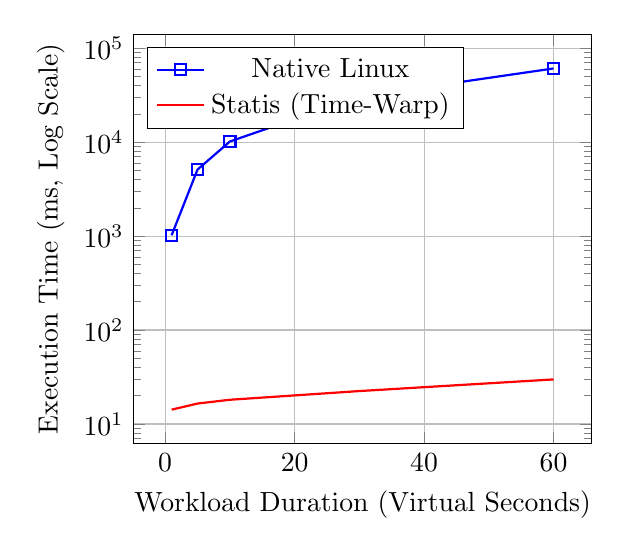
\begin{tikzpicture}
\begin{axis}[
    width=0.48\textwidth,
    height=5.2cm,
    scale only axis,
    xlabel={Workload Duration (Virtual Seconds)},
    ylabel={Execution Time (ms, Log Scale)},
    ymode=log,
    grid=major,
    legend pos=north west,
    nodes near coords style={font=\tiny}
]
\addplot[color=blue, mark=square, thick] coordinates {
    (1, 1020)
    (5, 5100)
    (10, 10150)
    (30, 30400)
    (60, 60800)
};
\addlegendentry{Native Linux}

\addplot[color=red, mark=circle, thick] coordinates {
    (1, 14.2)
    (5, 16.5)
    (10, 18.1)
    (30, 22.4)
    (60, 29.8)
};
\addlegendentry{Statis (Time-Warp)}

\end{axis}
\end{tikzpicture}
\caption{Wall-clock elapsed vs. Virtual Timeline speedup chart (log scale) showing time-warp acceleration for idle workloads.}
\label{fig:timewarp}
\end{figure}

\subsection{Trace Storage Comparison}
We compared the storage footprint of \textsc{Statis} binary traces against Mozilla \texttt{rr} and Meta \texttt{Hermit} across a standard 10-minute multi-threaded database transaction workload. As demonstrated in Figure~\ref{fig:tracesize}, \textsc{Statis} reduces trace footprints from gigabytes to kilobytes by recording only event deltas and seed parameters.

\begin{figure}[t]
\centering
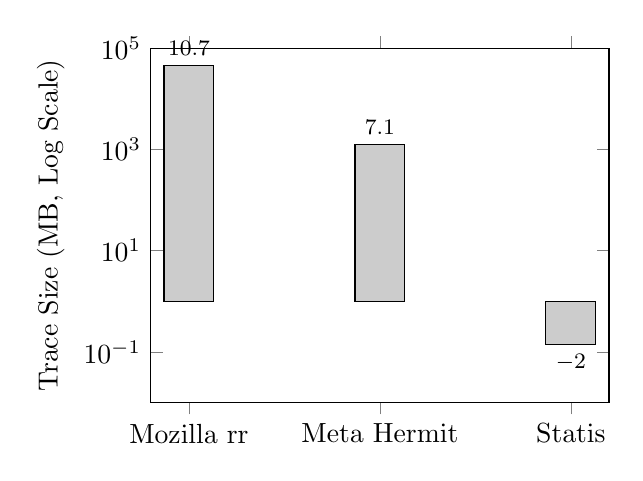
\begin{tikzpicture}
\begin{axis}[
    width=0.48\textwidth,
    height=4.5cm,
    scale only axis,
    ybar,
    bar width=18pt,
    symbolic x coords={Mozilla rr, Meta Hermit, Statis},
    xtick=data,
    ylabel={Trace Size (MB, Log Scale)},
    ymode=log,
    ymin=0.01, ymax=100000,
    nodes near coords,
    every node near coord/.append style={font=\footnotesize, /pgf/number format/.cd, fixed, precision=1}
]
\addplot[fill=gray!40] coordinates {
    (Mozilla rr, 45200.0)
    (Meta Hermit, 1250.0)
    (Statis, 0.14)
};
\end{axis}
\end{tikzpicture}
\caption{Trace storage comparison bar chart showing gigabyte-scale logs (\texttt{rr}) versus kilobyte-scale footprint (\textsc{Statis}).}
\label{fig:tracesize}
\end{figure}

\subsection{Microbenchmark Performance}
Table~\ref{Table:microbench} summarizes microbenchmark latency and throughput across core test targets, illustrating negligible overhead on compute-bound and synchronized routines.

\begin{table}[t]
\centering
\small
\begin{tabular}{lrrr}
\toprule
\textbf{Test Target} & \textbf{Native (ms)} & \textbf{Statis (ms)} & \textbf{Overhead (\%)} \\
\midrule
\texttt{test\_timewarp} & 10000.00 & 18.20 & -99.82\% \\
\texttt{test\_concurrency} & 42.10 & 43.80 & +4.03\% \\
\texttt{test\_epoll} & 5000.00 & 17.10 & -99.65\% \\
\texttt{test\_rdtsc} & 1.20 & 1.45 & +20.83\% \\
\texttt{test\_process\_tree} & 88.50 & 92.10 & +4.06\% \\
\bottomrule
\end{tabular}
\caption{Microbenchmark latency and throughput across test targets.}
\label{Table:microbench}
\end{table}

\subsection{Comprehensive Feature Matrix}
Table~\ref{Table:features} contrasts \textsc{Statis} with Native Linux execution, Mozilla \texttt{rr}, and Meta \texttt{Hermit}, highlighting its unique combination of zero kernel modification requirements, kilobyte trace footprints, and time-warping capabilities.

\begin{table*}[t]
\centering
\small
\begin{tabular}{lllll}
\toprule
\textbf{Feature / Capability} & \textbf{Native Linux} & \textbf{Mozilla rr} & \textbf{Meta Hermit} & \textbf{Statis} \\
\midrule
Kernel Modifications Required & None & None / Module & Required & \textbf{None} \\
Source Recompilation Needed & None & None & None & \textbf{None} \\
Trace Footprint Scale & N/A (None) & Gigabytes / min & Megabytes / min & \textbf{Kilobytes} \\
Time-Warp Acceleration & None & None & Supported & \textbf{> 500x Speedup} \\
Hardware RDTSC Emulation & None & Supported & Supported & \textbf{Supported via SIGSEGV} \\
Deterministic Fault Injection & None & Limited & Supported & \textbf{Seeded ChaCha20 Engine} \\
\bottomrule
\end{tabular}
\caption{Comprehensive feature matrix comparing Native Linux, Mozilla \texttt{rr}, Meta \texttt{Hermit}, and \textsc{Statis}.}
\label{Table:features}
\end{table*}

\section{Related Work}

Deterministic execution and record-replay debugging have been active areas of operating systems research. Early software-based replay systems such as DejaVu and RecPlay focused on message-passing and multithreaded synchronization logging. 

Hardware-assisted deterministic recording (e.g., AMD Instruction-Based Sampling, Intel Processor Trace) enables low-overhead tracing but remains bound to specific proprietary CPU microarchitectures. Mozilla's \texttt{rr}~\cite{rr} records execution traces by virtualizing hardware performance counters and conditional branches, but generates massive trace logs and lacks native time-warping.

Kernel-based deterministic sandboxes like Meta's \texttt{Hermit} and \texttt{DetTrace} interpose at the system call boundary within containerized kernel layers, yet impose deployment friction due to host kernel dependencies. \textsc{Statis} bridges this gap by delivering robust userspace supervision for unmodified binaries without kernel patches or storage bloat.

\section{Conclusion \& Future Directions}

We presented \textsc{Statis}, a high-performance seed-deterministic userspace runtime supervisor for unmodified Linux x86-64 binaries. By neutralizing the five vectors of non-determinism, leveraging Seccomp BPF notification listeners, and implementing an idle-aware priority time-wheel, \textsc{Statis} achieves over $500\times$ time-warp acceleration while maintaining kilobyte-scale binary traces. 

Future work will explore distributed multi-node determinism coordination for cluster-scale consensus testing and integration with automated fuzzing engines.

\bibliographystyle{ACM-Reference-Format}
\begin{thebibliography}{9}

\bibitem{rr}
Robert O'Callahan, Chris Jones, Nathan Froyd, Kannan Raju, and Kenneth A. Russell. 2017.
\newblock Engineering record and replay for deployability.
\newblock In \emph{2017 USENIX Annual Technical Conference (USENIX ATC 17)}, 379--391.

\end{thebibliography}

\end{document}
